\documentclass[a4paper,10pt,oneside]{jsbook}
%
\usepackage{amsmath,amssymb,bm}
\usepackage{bm}
\usepackage[dvipdfmx]{graphicx}
\usepackage{ascmac}
\usepackage{makeidx}
\usepackage{txfonts}
\usepackage{indentfirst}
\usepackage{booktabs}
\usepackage{tabularx}
\usepackage{comment}
\AtBeginDvi{\special {pdf:tounicode EUC-UCS2}}
\usepackage[dvipdfmx, setpagesize=false, bookmarks=true, bookmarksnumbered=true]{hyperref}
\usepackage{nameref}
\usepackage{url}
\usepackage{wrapfig}

%
\makeindex
%
\newcommand{\diff}{\mathrm{d}}            %微分記号
\newcommand{\divergence}{\mathrm{div}\,}  %ダイバージェンス
\newcommand{\grad}{\mathrm{grad}\,}       %グラディエント
\newcommand{\rot}{\mathrm{rot}\,}         %ローテーション
%
\setlength{\textwidth}{\fullwidth}
\setlength{\textheight}{44\baselineskip}
\addtolength{\textheight}{\topskip}
\setlength{\voffset}{-0.6in}
%

\begin{document}

%%%%%%%%%%%%%%%%%%%%%%%%%%%%%%%%%%%%%%%%%%%%%%%%%%%%%
% 表紙
\begin{titlepage}
\noindent
独立行政法人 理化学研究所 御中
\begin{center}
	\vspace{8cm}
	{\Huge \textbf{協調ワークスペースドライバと}} \\
	\vspace{1cm}
	{\Huge \textbf{協調動作フレームワークのプロトタイプ}} \\
	\vspace{1cm}
	{\Huge \textbf{操作説明書}} \\
	\vspace{10cm}
	{\Large \textbf{2015年3月26日}} \\
	\vspace{0.5cm}
	{\Large \textbf{株式会社イマジカ デジタルスケープ}}
\end{center}
\end{titlepage}



%%%%%%%%%%%%%%%%%%%%%%%%%%%%%%%%%%%%%%%%%%%%%%%%%%%%%
% 目次
\tableofcontents

%%%%%%%%%%%%%%%%%%%%%%%%%%%%%%%%%%%%%%%%%%%%%%%%%%%%%
% 本文
%%%%%%%%%%%%%%%%%%%%%%%%%%%%%%%%%%%%%%%%%%%%%%%%%%%%%
\chapter{はじめに}
本書では協調ワークスペースドライバと協調動作フレームワークのプロトタイプの操作方法について解説します.\\

\section{動作環境とインストール}
以下の環境で動作確認を行っております.\\

\begin{tabbing}
0123\=01234567890123\=0123456789\kill
\> OS \> : Linux, Windows(Vista,7,8), MacOSX \\
\> Webブラウザ \> :  Apple Safari 6.x, Firefox 33.0, Chrome 41, Internet Explorer 11
\end{tabbing}

\newpage

%%%%%%%%%%%%%%%%%%%%%%%%%%%%%%%%%%%%%%%%%%%%%%%%%%%%%
% アプリケーションの展開
%%%%%%%%%%%%%%%%%%%%%%%%%%%%%%%%%%%%%%%%%%%%%%%%%%%%%
\chapter{アプリケーションの展開方法}

アーカイブファイルの解凍を行ってください.\\
解凍すると、以下の構成でファイルが作成されます.\\

\begin{tabbing}
0123\=01234567890123\=0123456789\kill
\>bin        \> : 実行スクリプトフォルダ\\
\>client     \> : TDDクライアントアプリケーションフォルダ\\
\>doc        \> : ドキュメントフォルダ\\
\>redis      \> : redisアプリケーションフォルダ\\
\>server     \> : TDDサーバーアプリケーションフォルダ\\
\>package.json
\end{tabbing}

TiledDisplayDriverの起動にはbinフォルダに格納されているスクリプトを使用します.\\

\newpage

%%%%%%%%%%%%%%%%%%%%%%%%%%%%%%%%%%%%%%%%%%%%%%%%%%%%%
% インストール
%%%%%%%%%%%%%%%%%%%%%%%%%%%%%%%%%%%%%%%%%%%%%%%%%%%%%

\chapter{アプリケーションのインストール方法}

\section{インストール}

\subsection{Node.jsのインストール}
ポータルGUIの動作にはNode.jsのインストールが必要です.\\
Node.jsの公式サイト(\verb+http://nodejs.org/+)からNode.js本体をダウンロードし,インストールします.

\begin{figure}[htbp]
	\begin{center}
		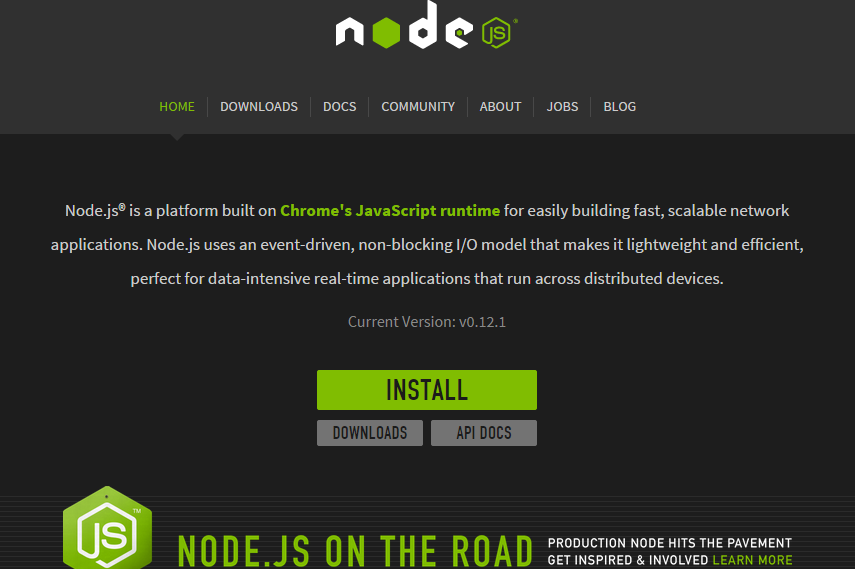
\includegraphics[width=15.5cm]{image/NodeJS.png}
	\end{center}
	\caption{node.jsのinstall画面}
	\label{fig:nodejs_home}
\end{figure}

\newpage


\subsection{Node.jsサブモジュールのインストール}
アプリケーションを展開したディレクトリに,
ポータルGUIで利用しているNode.jsの必要なサードパーティモジュールのインストールを行います.

\section{インストールスクリプトの実行}

\subsection{Mac/Linuxの場合}
bin配下の以下のシェルスクリプトを実行します.\\

\begin{verbatim}
   $cd bin
   $sh install.sh
\end{verbatim}


\subsection{Windowsの場合}
bin配下の以下のファイルを実行します.\\
\begin{verbatim}
   >cd bin
   >install.bat
\end{verbatim}

\newpage


%%%%%%%%%%%%%%%%%%%%%%%%%%%%%%%%%%%%%%%%%%%%%%%%%%%%%
% アプリケーションの起動方法
%%%%%%%%%%%%%%%%%%%%%%%%%%%%%%%%%%%%%%%%%%%%%%%%%%%%%
\chapter{アプリケーションの起動方法}


\subsection{Mac/Linuxの場合}
bin配下の以下のシェルスクリプトを実行します.\\
./run.sh

\subsection{Windowsの場合}
bin配下の以下のファイルを実行します.\\
\begin{verbatim}
   >cd bin
   >run.bat
\end{verbatim}


※
Windowsの場合、仮想メモリを0KByteにしていると、
redisが正常に起動しない場合があります.\\
その場合は一時的に仮想メモリを有効にしてご利用ください.\\

\newpage


%%%%%%%%%%%%%%%%%%%%%%%%%%%%%%%%%%%%%%%%%%%%%%%%%%%%%
% アプリケーションの起動確認
%%%%%%%%%%%%%%%%%%%%%%%%%%%%%%%%%%%%%%%%%%%%%%%%%%%%%
\section{起動確認}
起動スクリプトを実行するとポータルGUIサーバーが起動します.
\begin{verbatim}
   $sh run.sh
   (Windows版は run.bat)
\end{verbatim}

\section{コントローラへアクセス}
TDDへのアクセスは、Webブラウザのアドレス欄に「http://localhost:8080」と入力することでアクセス出来ます.\\
アクセスし、図\ref{fig:home}の画面が表示されたらインストールは完了となります。.\\

\begin{figure}[htbp]
	\begin{center}
		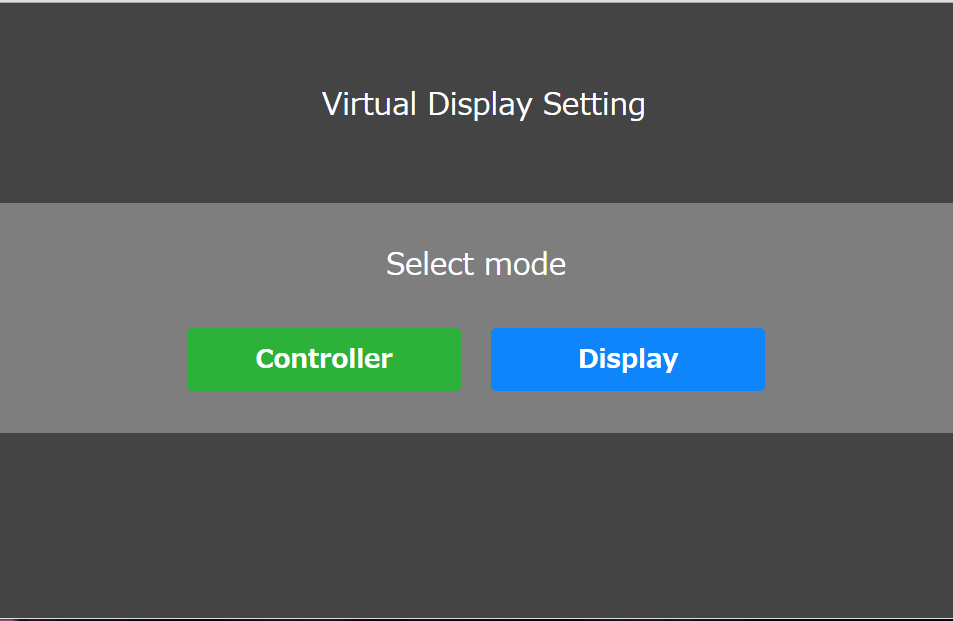
\includegraphics[width=15.5cm]{image/home.png}
	\end{center}
	\caption{insall終了後ホーム画面}
	\label{fig:home}
\end{figure}

\newpage

%%%%%%%%%%%%%%%%%%%%%%%%%%%%%%%%%%%%%%%%%%%%%%%%%%%%%
% アプリケーションの終了方法
%%%%%%%%%%%%%%%%%%%%%%%%%%%%%%%%%%%%%%%%%%%%%%%%%%%%%
\chapter{アプリケーションの終了方法}

以下2点の操作にて終了させます.\\

\subsection{サーバープログラムの終了}\
run.sh(bat)を起動したterminalをCTRL+Cで終了するか、
serverプログラムをkillします.\\


\subsection{redisの終了}
redisが起動しているterminalを終了させます.\\
また、プロセスとして起動している場合は、プロセスをpsコマンドにて見つけて
killコマンドにて終了させます.\\

\newpage

%%%%%%%%%%%%%%%%%%%%%%%%%%%%%%%%%%%%%%%%%%%%%%%%%%%%%
% TiledDisplayDriverのホーム画面
%%%%%%%%%%%%%%%%%%%%%%%%%%%%%%%%%%%%%%%%%%%%%%%%%%%%%
\chapter{TiledDisplayDriverのホーム画面}
\section{ホーム画面説明}
TiledDisplayDriver(以下TDDと略記)は、以下の2つのコントローラ(Display, Controller制御)側か、Display側かを決定します.\\
TDDへのアクセスは、前述のアプリケーション起動を行った後、Webブラウザのアドレス欄に「http://localhost:8080」と入力することでアクセス出来ます.\\
アクセスすると図\ref{fig:home}が表示されます.

\begin{itemize}
\item Controller: コントローラ画面へと遷移します.\\
\item Display   : ディスプレイ画面へと遷移します.\\
\end{itemize}

上記の通り、アクセスしたPCを「コントローラ」として使用するか、
「ディスプレイ」として使用するかを選択することができます.\\

\newpage


%%%%%%%%%%%%%%%%%%%%%%%%%%%%%%%%%%%%%%%%%%%%%%%%%%%%%
% コントローラ画面の操作
%%%%%%%%%%%%%%%%%%%%%%%%%%%%%%%%%%%%%%%%%%%%%%%%%%%%%
\chapter{コントローラ画面の操作}
\section{概要}
コントローラは\ref{controller}の通りとなっております.\\
\begin{figure}[htbp]
	\begin{center}
		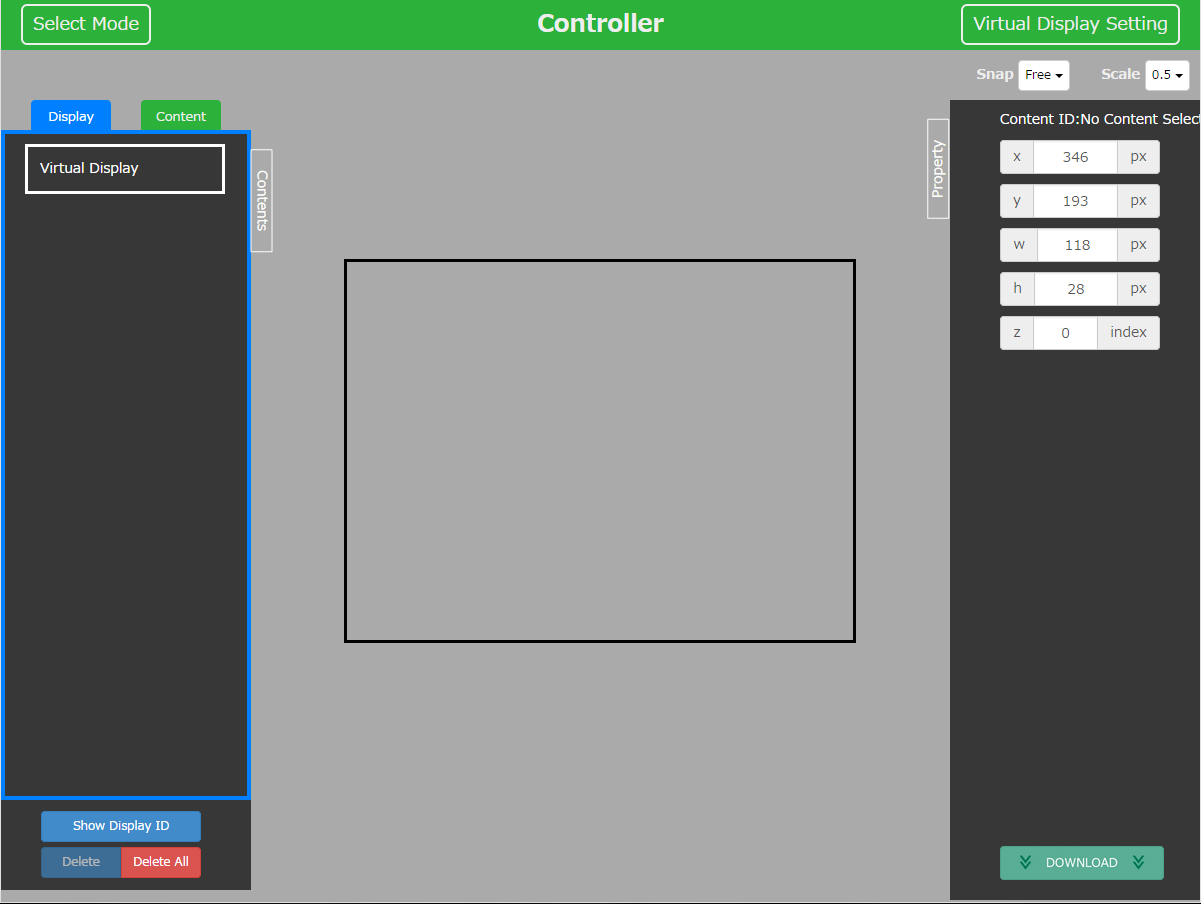
\includegraphics[width=15.5cm]{image/cont_1.PNG}
	\end{center}
	\caption{コントローラ画面概要}
	\label{fig:controller}
\end{figure}

それぞれのタブ、ウィンドウ等、機能について解説します.\\

\newpage


%%%%%%%%%%%%%%%%%%%%%%%%%%%%%%%%%%%%%%%%%%%%%%%%%%%%%
% コントローラ画面の操作
%%%%%%%%%%%%%%%%%%%%%%%%%%%%%%%%%%%%%%%%%%%%%%%%%%%%%
\section{コントローラの操作 : VirtualDisplayScreenについて}
中央はVirtualDisplayScreenと呼ばれ、TiledDisplayServerに接続された
ディスプレイの操作、コンテンツの移動、操作、削除等を行う
汎用スペースとなっております.\\

\begin{figure}[htbp]
	\begin{center}
		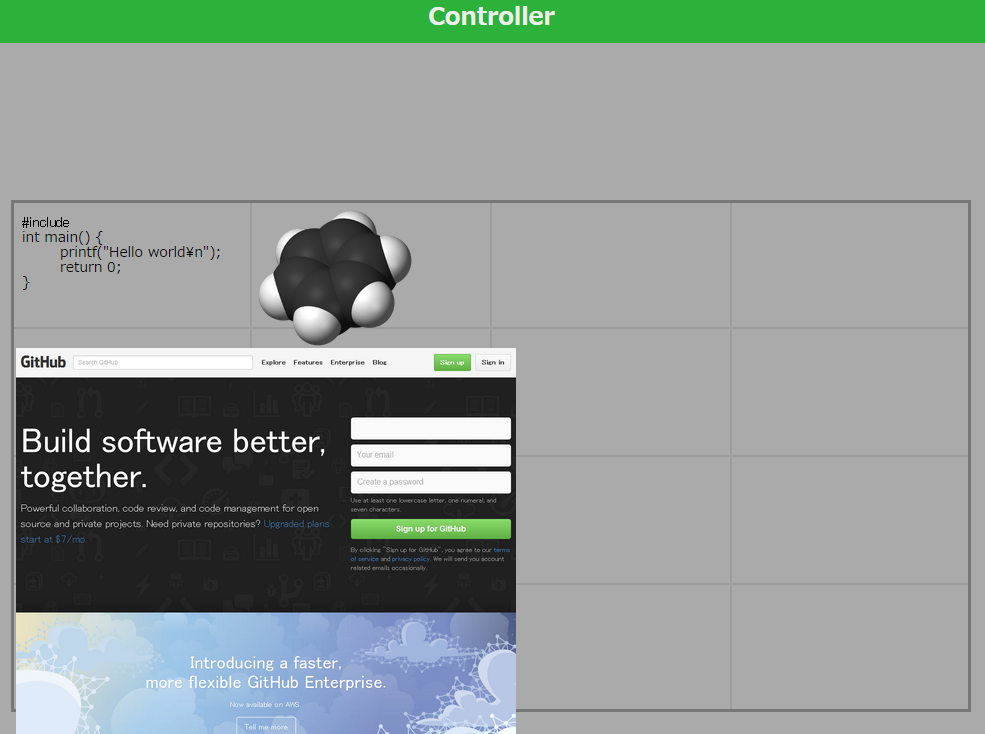
\includegraphics[width=15.5cm]{image/TDD_View.PNG}
	\end{center}
	\caption{VirtualDisplayScreenの凡例}
	\label{fig:vds}
\end{figure}

\newpage



%%%%%%%%%%%%%%%%%%%%%%%%%%%%%%%%%%%%%%%%%%%%%%%%%%%%%
% コントローラ画面の操作
%%%%%%%%%%%%%%%%%%%%%%%%%%%%%%%%%%%%%%%%%%%%%%%%%%%%%
\section{コントローラの操作 : Contentsタブ(Displayタブ)}
\begin{wrapfigure}{r}{60mm}
	\begin{center}
		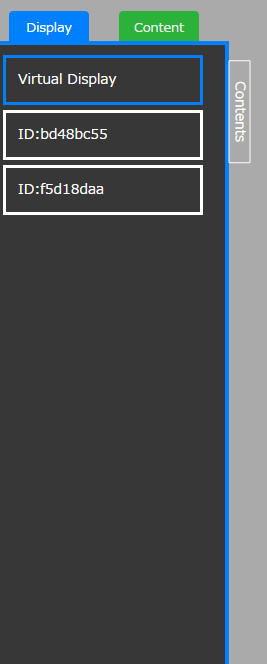
\includegraphics[width=5.5cm]{image/Display_TAB_2conn.PNG}
	\end{center}
	\caption{Contentsタブ(Displayタブ)}
	\label{fig:contentstab}
\end{wrapfigure}

VirtualDisplayと、TDDサーバーに接続されているDisplayの一覧を表示します.\\
コントローラは、このDisplayをVirtualDisplay上に配置することができます.\\

配置したDisplay上にコンテンツを追加することによってコンテンツを共有するワークスペースを実現します.\\
Displayはマウスドラッグドロップにより、VirtualDisplaySpaceに配置することができます.\\
\\ 
図\ref{fig:contentstab}は、2クライアントが接続された環境の例となります.


\clearpage 



%%%%%%%%%%%%%%%%%%%%%%%%%%%%%%%%%%%%%%%%%%%%%%%%%%%%%
% sub snap機能
%%%%%%%%%%%%%%%%%%%%%%%%%%%%%%%%%%%%%%%%%%%%%%%%%%%%%
\subsection{snap機能}
Displayを正確に区画に配置するための機能として「snap機能」があります.\\
図\ref{fig:snapdisp}のボタンとなります.\\

\begin{figure}[htbp]
	\begin{center}
		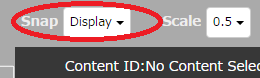
\includegraphics[width=5.5cm]{image/MIGIUE_Disp.PNG}
	\end{center}
	\caption{Snap機能の設定プルダウンボタン}
	\label{fig:snapdisp}
\end{figure}


\begin{tabbing}
0123\=01234567890123\=0123456789\kill
\>Free    \> : 自由配置となります.\\
\>Display \> : 分割した区画に沿ってDisplay及びコンテンツがスナップするようになります.
\end{tabbing}

図\ref{fig:snapdrag}にsnap機能を用いて配置する凡例を示します。.\\

\begin{figure}[htbp]
	\begin{center}
		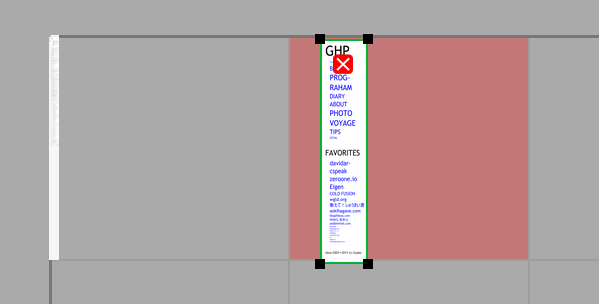
\includegraphics[width=15.5cm]{image/Snap1.png}
	\end{center}
	\caption{Snap機能ドラッグ時凡例}
	\label{fig:snapdrag}
\end{figure}

\clearpage 

またVirtualDisplaySpaceの拡大縮小オプションとして、Scale機能があります。図\ref{fig:scale}のボタンとなります.\\

\begin{figure}[htbp]
	\begin{center}
		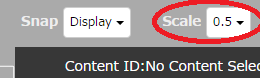
\includegraphics[width=7.5cm]{image/MIGIUE_Scale.PNG}
	\end{center}
	\caption{scale機能}
	\label{fig:scale}
\end{figure}

デフォルトは0.5となっております.\\



\clearpage 


%%%%%%%%%%%%%%%%%%%%%%%%%%%%%%%%%%%%%%%%%%%%%%%%%%%%%
% sub Show Display IDボタン
%%%%%%%%%%%%%%%%%%%%%%%%%%%%%%%%%%%%%%%%%%%%%%%%%%%%%
\subsection{Show Display IDボタン}
接続されたDisplayのIDを各接続されたDisplay上に表示し、識別できるようにします.\\
尚、IDは、接続された端末固有であり、1端末につき1IDが割り当てられます.\\
\begin{figure}[htbp]
	\begin{center}
		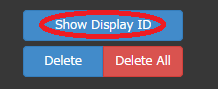
\includegraphics[width=7.5cm]{image/3Button1.PNG}
	\end{center}
	\caption{Show Display ID}
	\label{fig:showdisplayid}
\end{figure}


%%%%%%%%%%%%%%%%%%%%%%%%%%%%%%%%%%%%%%%%%%%%%%%%%%%%%
% sub Deleteボタン
%%%%%%%%%%%%%%%%%%%%%%%%%%%%%%%%%%%%%%%%%%%%%%%%%%%%%
\subsection{Delete}
選択したDisplayを削除(TDDサーバーから切断)します.\\
\begin{figure}[htbp]
	\begin{center}
		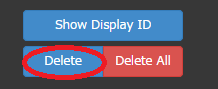
\includegraphics[width=7.5cm]{image/3Button2.PNG}
	\end{center}
	\caption{Deleteボタン}
	\label{fig:deletebutton}
\end{figure}

※尚、VirtualDisplayは削除することはできません.\\



%%%%%%%%%%%%%%%%%%%%%%%%%%%%%%%%%%%%%%%%%%%%%%%%%%%%%
% sub DeleteAllボタン
%%%%%%%%%%%%%%%%%%%%%%%%%%%%%%%%%%%%%%%%%%%%%%%%%%%%%
\subsection{Delete\ Allボタン}
接続されているDisplayすべてを削除(TDDサーバーから切断)します.\\

\begin{figure}[htbp]
	\begin{center}
		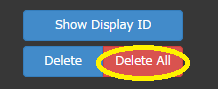
\includegraphics[width=7.5cm]{image/3Button3.PNG}
	\end{center}
	\caption{Delete\ Allボタン}
	\label{fig:deleteallbutton}
\end{figure}

\newpage


%%%%%%%%%%%%%%%%%%%%%%%%%%%%%%%%%%%%%%%%%%%%%%%%%%%%%
% sub コントローラの操作
%%%%%%%%%%%%%%%%%%%%%%%%%%%%%%%%%%%%%%%%%%%%%%%%%%%%%
\section{コントローラの操作 : 左(contentsタブ)}
本アプリケーションでは, ディスプレイへのコンテンツの表示は, 左側のコンテンツタブからディスプレイにコンテンツをドラッグアンドドロップすることにより行います.

\subsection{コンテンツの表示}
コンテンツ一覧から, 中央のVirtualScreenの領域へ, ドラッグアンドドロップすることで, 表示させることができます.\\

\begin{figure}[htbp]
	\begin{center}
		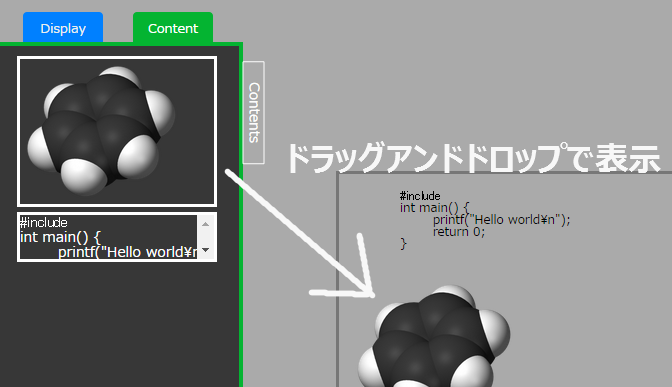
\includegraphics[width=11.5cm]{image/DragAndDropContent.png}
	\end{center}
	\caption{コンテンツの表示}
	\label{fig:draganddropcontent}
\end{figure}

\subsection{コンテンツ一覧への追加}
コンテンツの追加を行います.\\
Addボタンを押下することで, Add\ Contentウィンドウを開きます



%%%%%%%%%%%%%%%%%%%%%%%%%%%%%%%%%%%%%%%%%%%%%%%%%%%%%
% sub テキストファイルの追加
%%%%%%%%%%%%%%%%%%%%%%%%%%%%%%%%%%%%%%%%%%%%%%%%%%%%%
\subsection{テキストファイルの追加}
Add\ Contentポップアップからテキストファイルをコンテンツに追加します.\\
以下追加例となります.\\

\begin{figure}[htbp]
	\begin{center}
		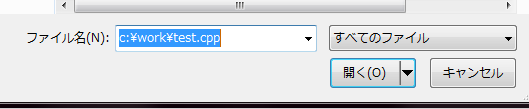
\includegraphics[width=11.5cm]{image/AddContent_TextFile_Select.png}
	\end{center}
	\caption{テキストファイルを選択}
	\label{fig:addtext}
\end{figure}


\begin{figure}[htbp]
	\begin{center}
		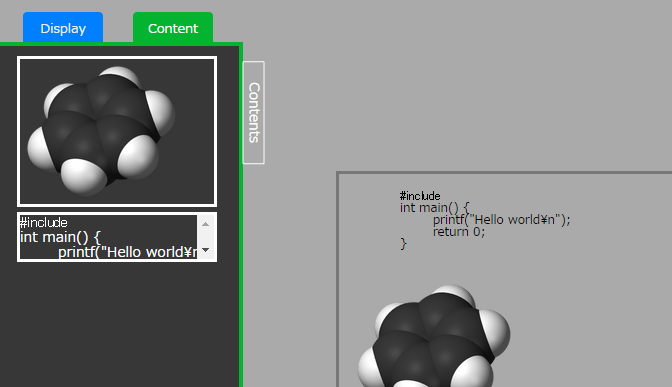
\includegraphics[width=15.5cm]{image/AddContent_TextFile_View.png}
	\end{center}
	\caption{テキストファイルのVirtualScreenへの追加}
	\label{fig:addtextfile}
\end{figure}

\newpage



%%%%%%%%%%%%%%%%%%%%%%%%%%%%%%%%%%%%%%%%%%%%%%%%%%%%%
% sub URLの送信
%%%%%%%%%%%%%%%%%%%%%%%%%%%%%%%%%%%%%%%%%%%%%%%%%%%%%
\subsection{URLの送信}
Contentポップアップから入力されたURLのサイトの画像をコンテンツに追加します.\\
以下例となります.\\
\begin{figure}[htbp]
	\begin{center}
		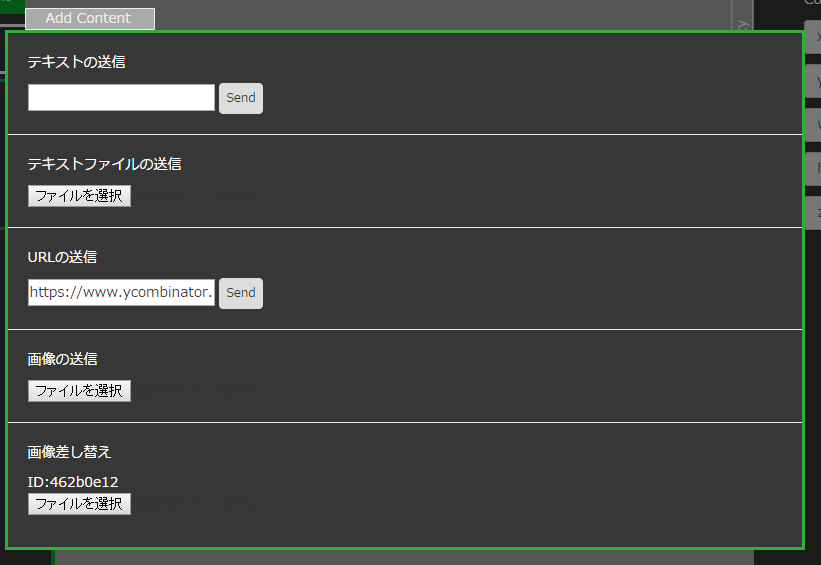
\includegraphics[width=12.5cm]{image/AddContent_URL.PNG}

	\end{center}
	\caption{URL送信ボタン}
	\label{fig:urlsend}
\end{figure}

追加すると以下の通りとなります.\\


\begin{figure}[htbp]
	\begin{center}
		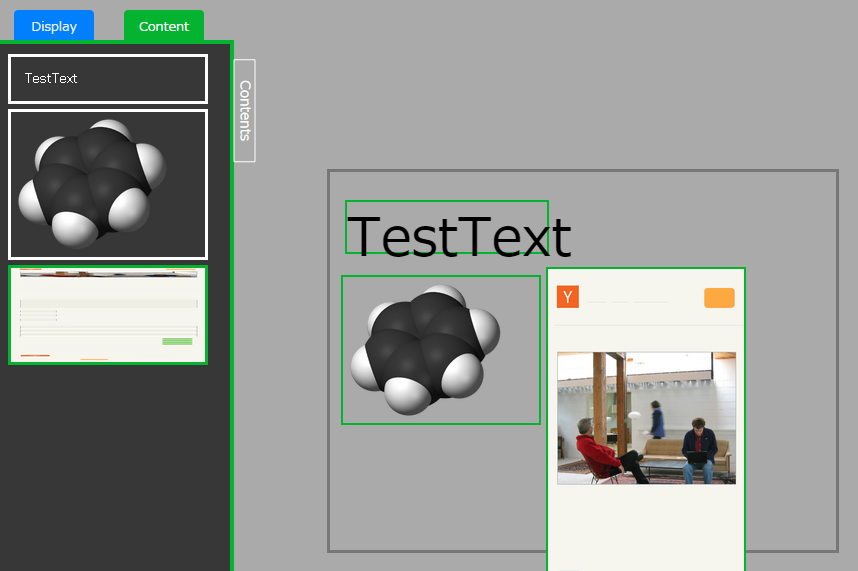
\includegraphics[width=12.5cm]{image/AddContent_URL_View.PNG}
	\end{center}
	\caption{URL送信後View}
	\label{fig:sendurl}
\end{figure}

\newpage





%%%%%%%%%%%%%%%%%%%%%%%%%%%%%%%%%%%%%%%%%%%%%%%%%%%%%
% sub 画像の送信
%%%%%%%%%%%%%%%%%%%%%%%%%%%%%%%%%%%%%%%%%%%%%%%%%%%%%
\subsection{画像の送信}
Contentポップアップから任意の画像ファイルをコンテンツに追加します.\\
対応している画像フォーマットは以下の通りです.\\

\begin{itemize}
\item PNGフォーマット形式.
\item JPEGフォーマット形式.
\end{itemize}

以下は表示例となります.\\
\begin{figure}[htbp]
	\begin{center}
		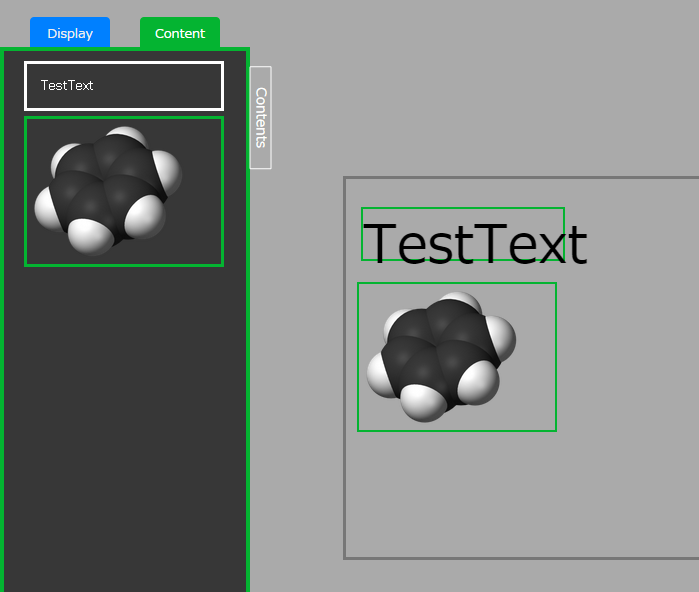
\includegraphics[width=11.5cm]{image/AddContent_Picture_View.PNG}
	\end{center}
	\caption{画像の追加凡例}
	\label{fig:addimage}
\end{figure}



\newpage

%%%%%%%%%%%%%%%%%%%%%%%%%%%%%%%%%%%%%%%%%%%%%%%%%%%%%
% sub 画像の差し替え
%%%%%%%%%%%%%%%%%%%%%%%%%%%%%%%%%%%%%%%%%%%%%%%%%%%%%
\subsection{画像の差し替え}
contentsタブにて選択している画像の差し替えを行います.\\
差し替え例を以下に示します.\\

\begin{figure}[htbp]
	\begin{center}
		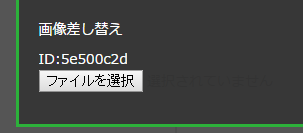
\includegraphics[width=11.5cm]{image/SASHI.PNG}
	\end{center}
	\caption{画像の差し替えボタン}
	\label{fig:replaceimagebutton}
\end{figure}

図\ref{fig:replaceimage}の通り指定すると、コンテンツタブに存在するコンテンツが差し替わります。\\

\begin{figure}[htbp]
	\begin{center}
		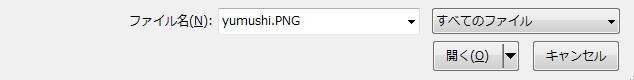
\includegraphics[width=11.5cm]{image/YUMUSHI.PNG}
	\end{center}
	\caption{画像の差し替え凡例}
	\label{fig:replaceimage}
\end{figure}


\begin{figure}[htbp]
	\begin{center}
		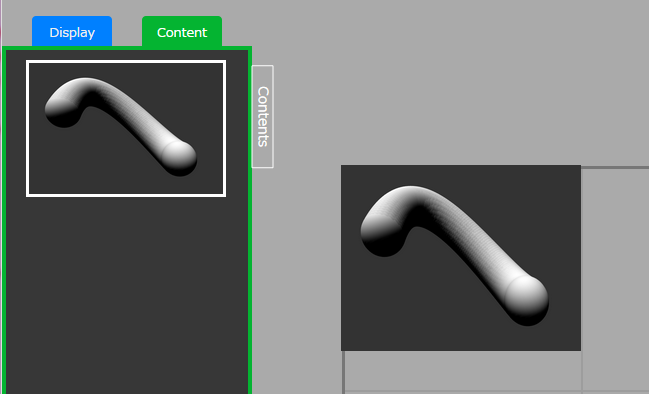
\includegraphics[width=11.5cm]{image/SASHI2.PNG}
	\end{center}
	\caption{画像の差し替え結果}
	\label{fig:replaceimageresult}
\end{figure}




\clearpage 

%%%%%%%%%%%%%%%%%%%%%%%%%%%%%%%%%%%%%%%%%%%%%%%%%%%%%
% プロパティタブ
%%%%%%%%%%%%%%%%%%%%%%%%%%%%%%%%%%%%%%%%%%%%%%%%%%%%%
\chapter{コントローラの操作 : propartyウィンドウ }
\begin{wrapfigure}{r}{60mm}
	\begin{center}
		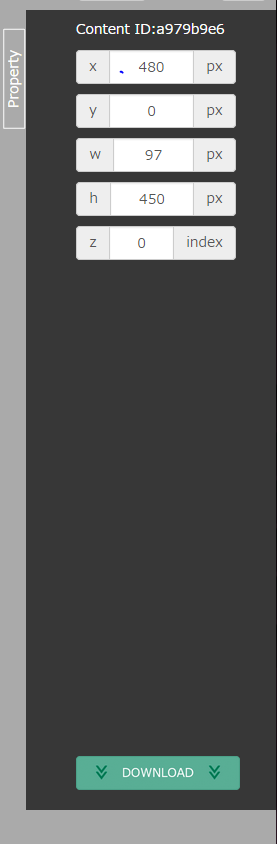
\includegraphics[width=5.5cm]{image/Prop_Down.PNG}
	\end{center}
	\caption{propartyウィンドウ}
	\label{fig:propall}
\end{wrapfigure}

propartyウィンドウは選択されたコンテンツ、Display、ContentsのID、
およびそれぞれのpropartyを表示します.\\

propartyは以下の通りID以外を編集し、座標、表示全面の優先順位 Zindex を
指定することができます.\\


また、選択されたContentsはpropartyウィンドウ左下のダウンロードボタンから
ダウンロードすることができます.\\


\clearpage 



%%%%%%%%%%%%%%%%%%%%%%%%%%%%%%%%%%%%%%%%%%%%%%%%%%%%%
% コントローラの操作 : 上記操作
%%%%%%%%%%%%%%%%%%%%%%%%%%%%%%%%%%%%%%%%%%%%%%%%%%%%%
\chapter{コントローラの操作 : 上部表示領域}
\subsection{SelectModeボタン}
SelectModeボタンは、再びホーム画面に戻るボタンとなります。

\begin{figure}[htbp]
	\begin{center}
		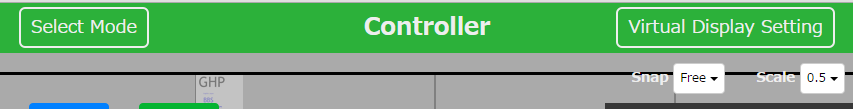
\includegraphics[width=8.5cm]{image/Upper.PNG}
	\end{center}
	\caption{画面上部領域}
	\label{fig:upperarea}
\end{figure}


\subsection{Virtual Display Settingボタン}

\begin{figure}[htbp]
	\begin{center}
		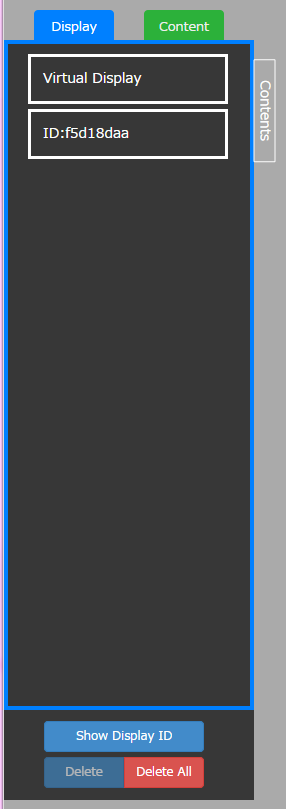
\includegraphics[width=8.5cm]{image/Left_Display.PNG}
	\end{center}
	\caption{Virtual Display Settingボタン押下時フォーカス}
	\label{fig:vdsfocus}
\end{figure}




Virtual Display Settingボタンを押下すると、Displayタブに操作をフォーカスします.\\



\clearpage 



\end{document}
